% Appendix:
\appendix

% Anexo A: Instrument
\section{Instrument}
\label{app:instrument}

As shown in Figure~\ref{fig:Figure2}, these results are impressive. \lipsum[20]

\begin{figure}[ht]
  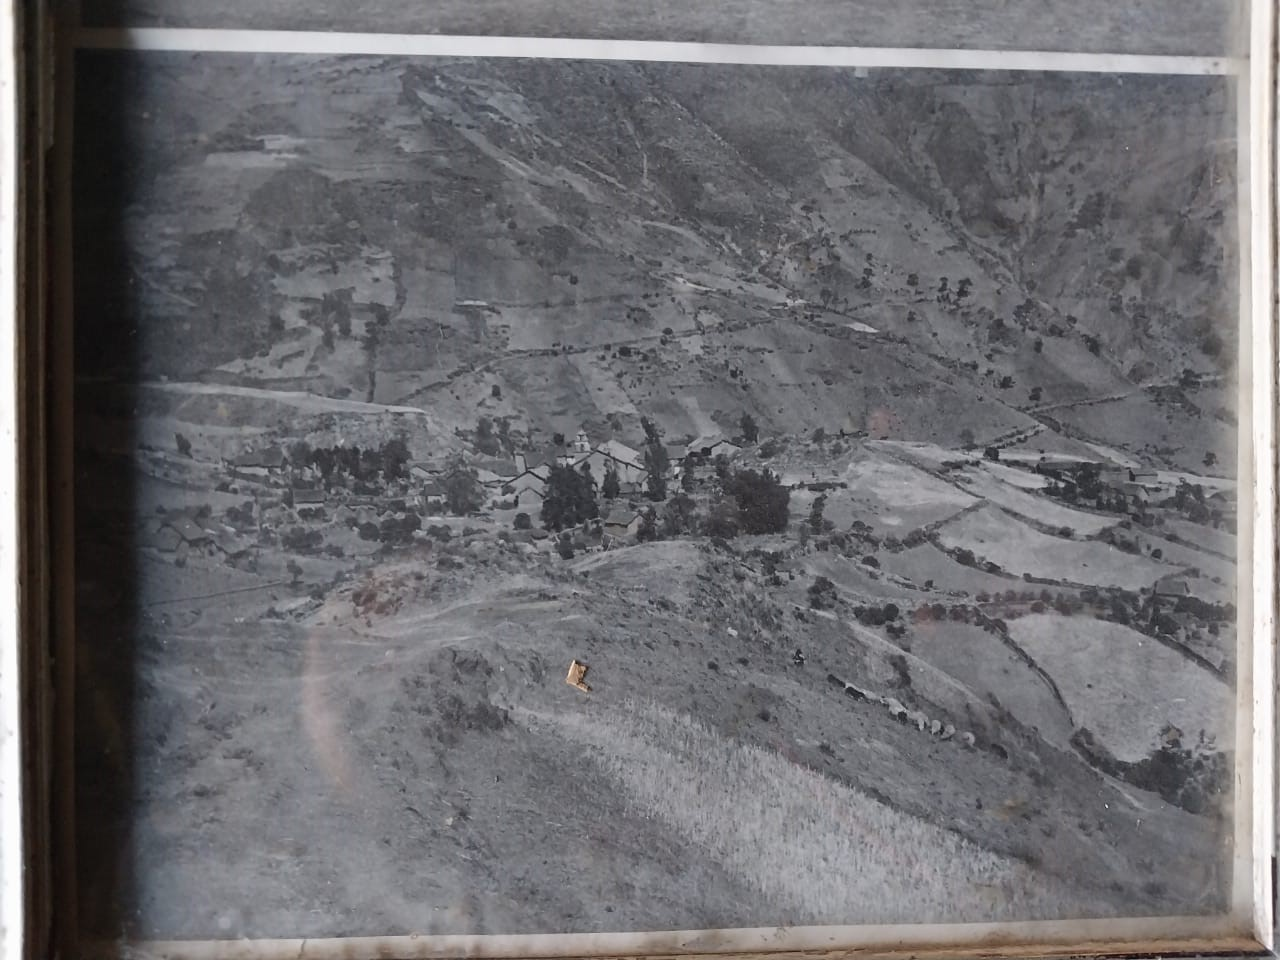
\includegraphics[scale=0.36]{F_Figures/15_Chapter VI/Cap6_Imagen2.jpeg}
	\caption{Cuadro y gráficos que muestran el método N2. Adaptado de \cite{deWaal2009}}
  \figurenote{This is a great figure.}
	\label{fig:Figure2}
\end{figure}

\lipsum[21]
% Pilot Data

\section{Pilot Data}
\label{app:surveydata}

The detailed results are shown in Table~\ref{tab:DeckedTable} from Anexo~\ref{app:surveydata}.

\lipsum[23]

\begin{table}[ht]
  \begin{threeparttable}
    \caption{A More Complex Decked Table}
    \label{tab:DeckedTable}
    \begin{tabular}{@{}lrrr@{}}         \toprule
    Distribution type  & \multicolumn{2}{l}{Percentage of} & Total number   \\
                       & \multicolumn{2}{l}{targets with}  & of trials per  \\
                       & \multicolumn{2}{l}{segment in}    & participant    \\ \cmidrule(r){2-3}
                                    &  Onset  &  Coda            &          \\ \midrule
    Categorical -- onset\tabfnm{a}  &    100  &     0            &  196     \\
    Probabilistic                   &     80  &    20\tabfnm{*}  &  200     \\
    Categorical -- coda\tabfnm{b}   &      0  &   100\tabfnm{*}  &  196     \\ \midrule
    \end{tabular}
    \tablenote{All data are approximate.

            \tabfnt{a}Categorical may be onset.
            \tabfnt{b}Categorical may also be coda.

            \tabfnt{*}\textit{p} < .05.
            \tabfnt{**}\textit{p} < .01.
         }
  \end{threeparttable}
\end{table}

\lipsum[23]